%\section{Tidsplan}
%\label{bilag1}
%\begin{figure}[H]
%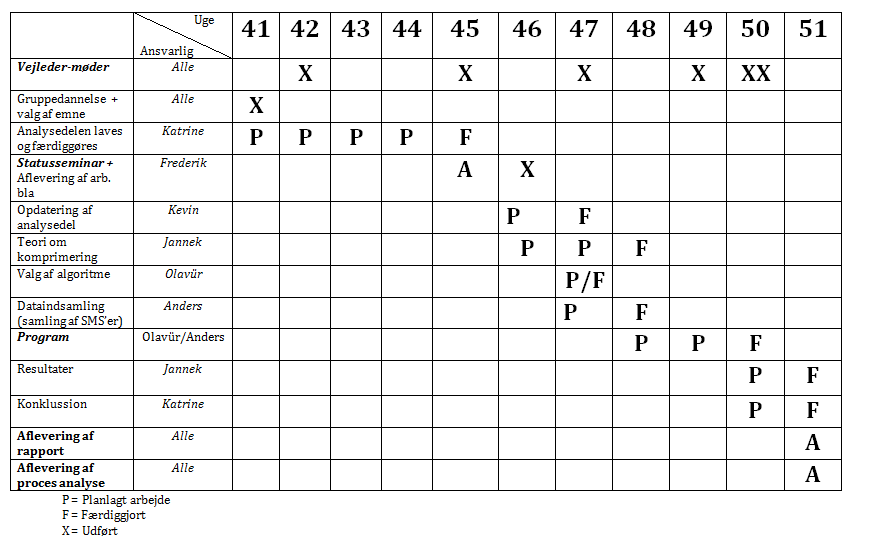
\includegraphics[width=\textwidth]{Indhold/tidsplan.png}
%\caption {Tidsplanen for projektet}
%\label {tidsplan}
%\end{figure}

\section{Arbejdsintensitet på GitHub}
\label{bilag2}
\begin{figure}[H]
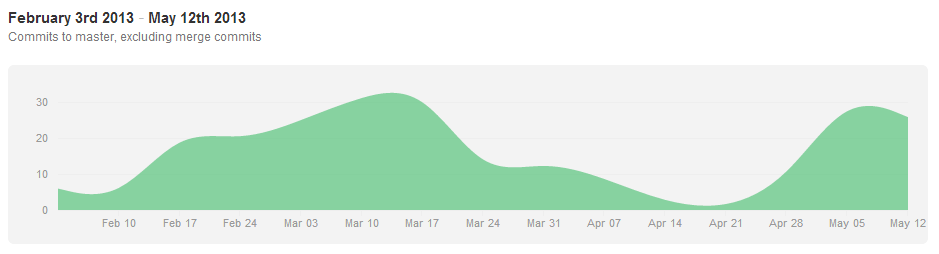
\includegraphics[width=\textwidth]{Indhold/arbejdsintensitet.png}
\caption {Billedet viser hvor ofte vi har "commitet" nye filer eller nyt arbejde til vores fælles mappe}
\label {arbejde}
\end{figure}


\section{Eksempel på referat fra vejledermøde}

Torsdag 4 April
Dagsorden:
1. Objekt orienteret Analyse og design
2. Spørgsmål til Lones kommentarer
3. Spørgsmål til kilder
4. Facebookside som kilde
5. Evt.
6. Næste møde
Generelt
1. Kommentarer til gruppens pdf er ikke klar endnu, men kommer snarest muligt.
2. Introduktion til Brugergrænseflader blev udskudt en uge grundet tekniske problemer.
3. Igen en smule forvirring over kildehenvisninger. Hvis henvisningen står ved en sætning
FØR punktummet, er det den specifikke sætning eller udsagn, som dokumenteres. Hvis
henvisningen står EFTER punktummet, henvises der til, at afsnittet har den givne kilde.
Objekt orienteret Analyse og Design:
1. Der var ikke nogle egentlige spørgsmål. Vi blev i gruppen enige om, at vi bare skal kaste
os ud i det, og så spørge hvis der er noget vi er i tvivl om.
Spørgsmål til Lones kommentarer
1. Hvordan skal vi vise at interessen for et emne var størst i en tidsperiode, men uden at det
står specifikt i en kilde? Vi kan samle flere kilder i et bilag og henivise til bilaget.
2. De fleste af Lones kommentarer er allerede blevet rettet.
3. Mange gange har Lone skrevet at vi skal omformulere. Dette er der ikke blevet gået så
meget op i indtil nu. Dette vil blive rettet hen mod slutningen af P2, hvor vejleder også vil
gå mere aktivt ind i det sproglige aspekt af rapporten.
4. Henvisninger til andre afsnit i Rapporten er fint at have som “Afsnit 3.2” for at dække os
ind mod senere omrokering af afsnittene.
Facebookside som kilde
1. En af vores kilder er en nyhed på en facebookside
(Danske Banks egen side). Er det en
lødig kilde? Det er nok ikke helt godt at henvise til Facebook, vi kan prøve at skrive til
DanskeBank og spørge, om de ikke har en pressemeddelelse vedr deres nye Layout.
Evt.
Når vi går i gang med at skrive programmet i OOP, skal vi bare kaste os ud i det. Vi skal ikke
være bange for at prøve noget, og så smide det helt væk og starte forfra.
Bøger:
1. Refactoring Martin
Fowler
2. Desgin patterns http://
en.wikipedia.org/wiki/Design_Patterns
3. The elements of LANGUAGE style evt.
http://www.amazon.com/TheElementsStyleKennethBaldwin/
dp/0521671590
Søge på c2wiki:
http://c2.com/cgi/wiki?FindPage
Næste møde
Torsdag 11 April, formentlig omkring 9:00